% -*- coding: utf-8 -*-
\section{ATH-kurve}
Average Threshold of Hearing (ATH) beskriver den mindste lydstyrke det menneskelige øre kan opfatte i de forskellige frekvensområder. Et plot af ATH for forskellige aldersgrupper vises i figur \ref{fig.ath}. Vores tilnærmede funktion beregnes som

ath(f) = 
-log10(f) * 0.2775 + 1 hvis f = 20 ...4000
0.0000625 * freq - 0.25, hvis f 4000 ... 20000  
1 ellers

og er vist i figur \ref{fig.vores-ath}.


\begin{figure}[h!]
\begin{center}
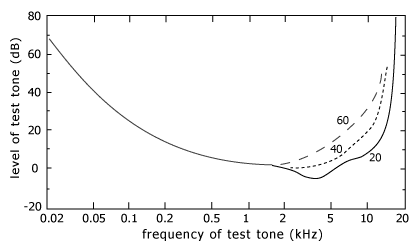
\includegraphics[width=12cm]{ATH}
\end{center}
\caption{Average Threshold of Hearing}
\label{fig.ath}
\end{figure}

\begin{figure}[h!]
\begin{center}
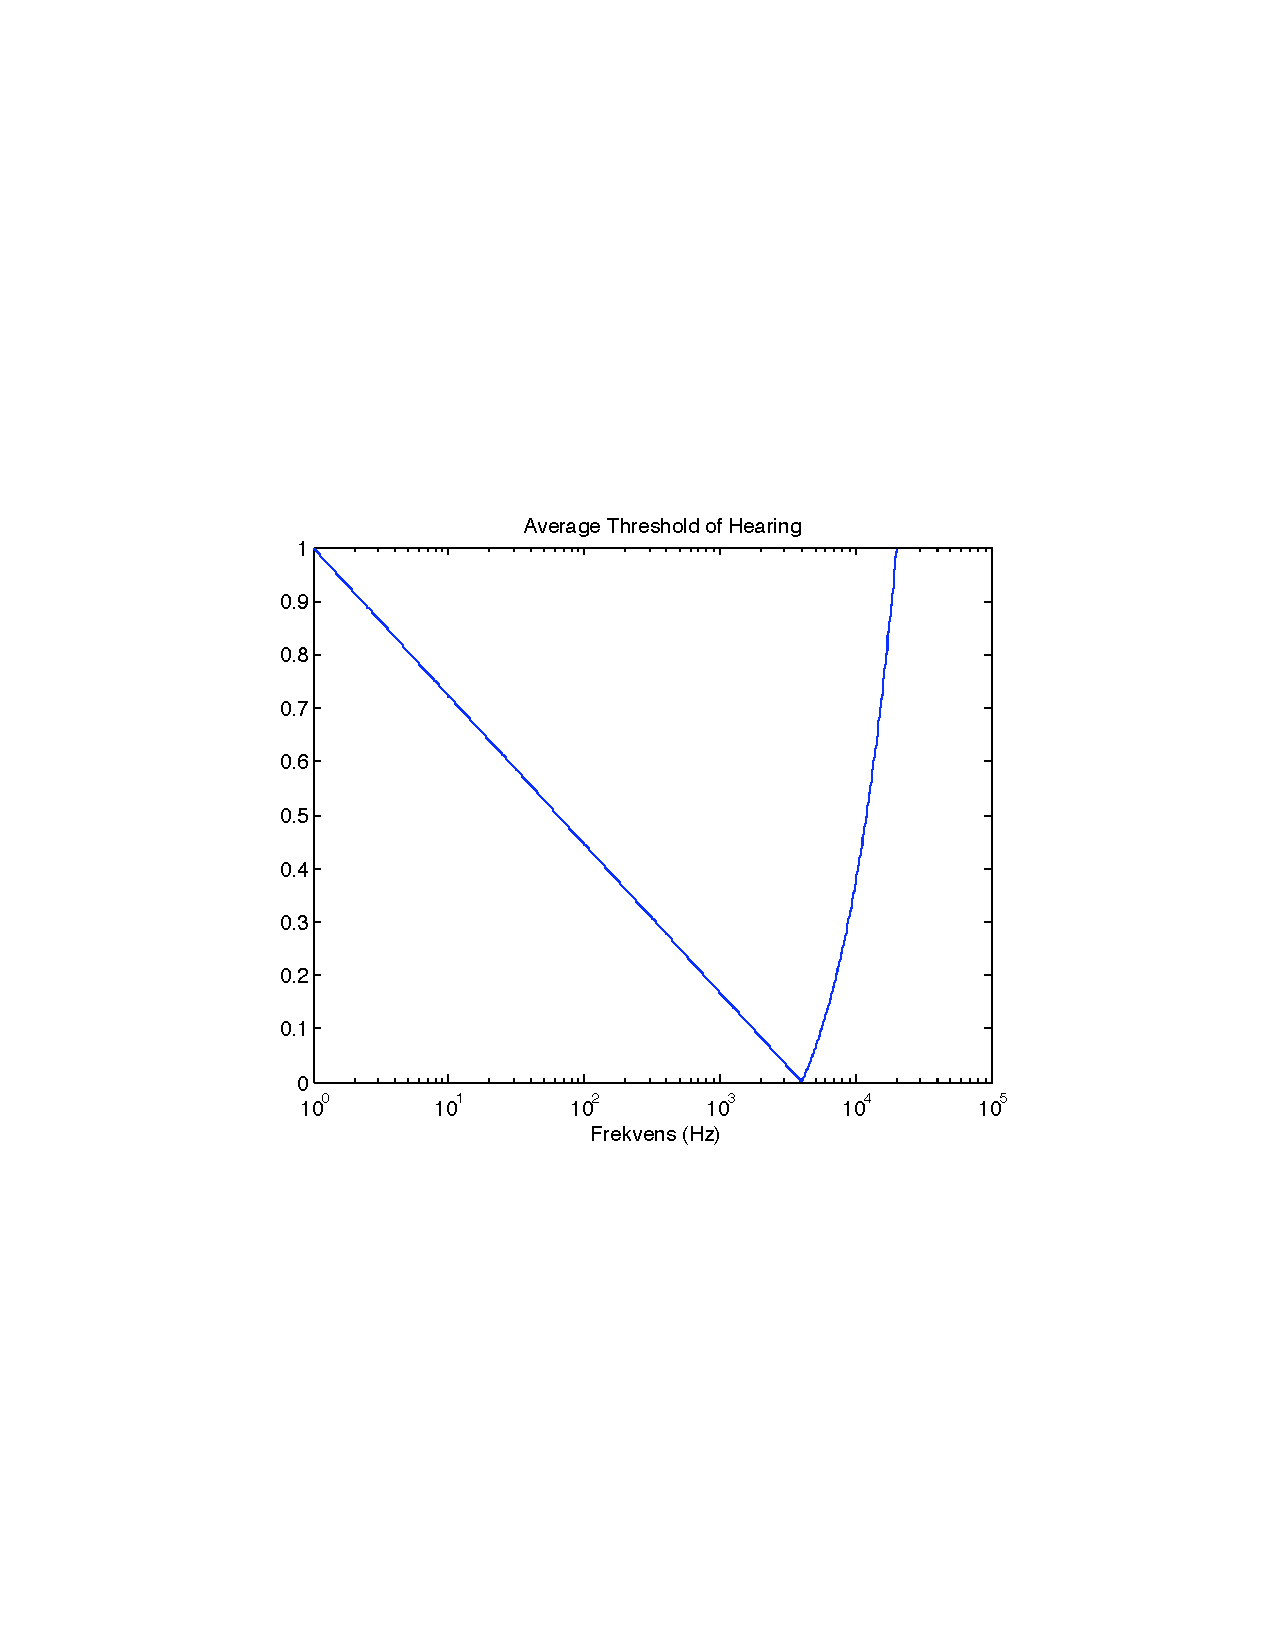
\includegraphics[width=12cm]{vores-ath}
\end{center}
\caption{Vores tilnærmede funktion til Average Threshold of Hearing}
\label{fig.vores-ath}
\end{figure}

